\chapter{Введение}
\markboth{\uppercase{Введение}}{\uppercase{Введение}}
\label{chap:introduction}

Нейронные сети стали неотъемлемой частью нашего повседневного мира, будь то в явном виде (например, в виде \textbf{больших языковых моделей}, БЯМ) или в скрытом, обеспечивая работу и расширяя возможности бесчисленных технологий и научных открытий \cite{wang2023scientific}, включая дроны, автомобили, поисковые системы, молекулярный дизайн и рекомендательные системы. Как мы увидим, все это было сделано с опорой на очень небольшой набор руководящих принципов и компонентов, составляющих ядро этой книги, в то время как исследовательский фокус сместился на их масштабирование до пределов физически возможного.

Сила масштабирования воплощена в относительно недавней концепции \textbf{нейронных законов масштабирования}, которая привела к огромным инвестициям в искусственный интеллект (ИИ) \cite{kaplan2020scaling,ho2024algorithmic}: неформально говоря, практически для любой задачи одновременное увеличение данных, вычислительной мощности и размера моделей — почти всегда — приводит к \textit{предсказуемому} повышению точности. Иными словами, вычислительная мощность, необходимая для достижения заданной точности для задачи, уменьшается на постоянный коэффициент за определенный период времени \cite{ho2024algorithmic}. Огромная мощь сочетания простых, универсальных инструментов с экспоненциально возросшей вычислительной мощностью в ИИ была названа Р. Саттоном \textit{горьким уроком}.\footnote{Р. Саттон, \textit{The Bitter Lesson}, \url{http://www.incompleteideas.net/IncIdeas/BitterLesson.html}.}

\begin{figure}
    \centering
    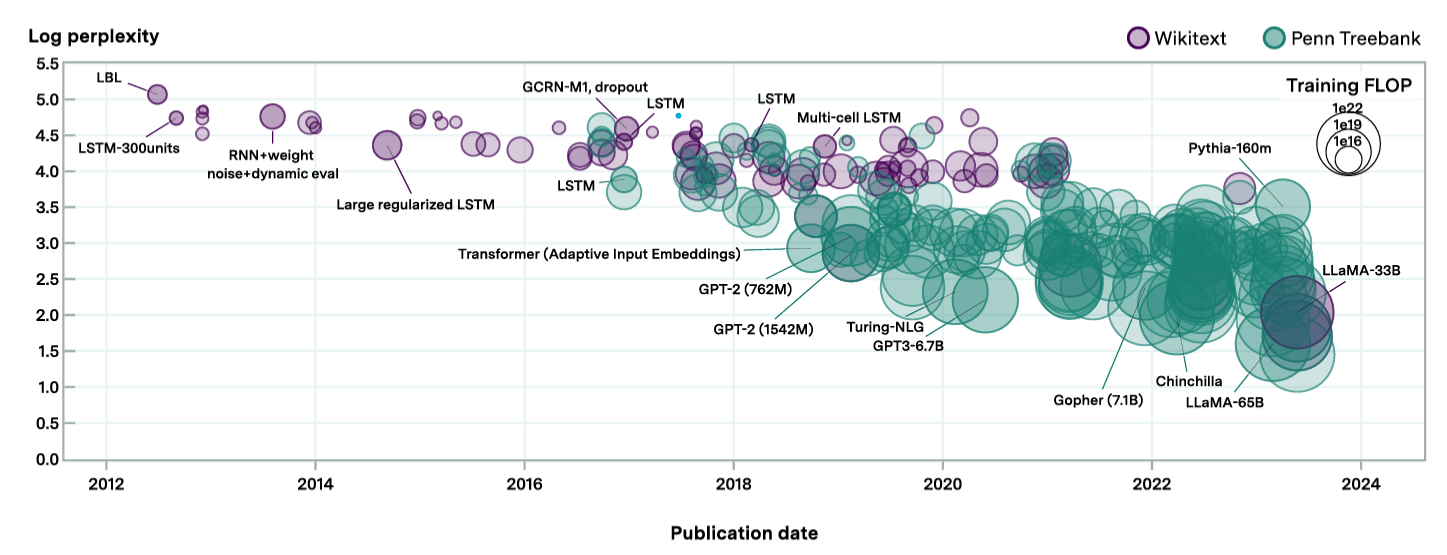
\includegraphics[width=0.9\textwidth]{images/compute_scaling.png}
    \caption{Производительность в \textbf{языковом моделировании} — предсказании продолжения предложения — здесь оцениваемая в терминах \textbf{перплексии}, неуклонно улучшалась, в то время как размер моделей постоянно увеличивался. Увеличение производительности также сопровождается эквивалентным масштабированием данных, при этом вариации в моделировании становятся асимптотически менее значимыми. Воспроизведено из \cite{ho2024algorithmic}.}
    \label{fig:compute_scaling}
\end{figure}

Если мы принимаем законы масштабирования как данность, у нас остается почти волшебный инструмент. В двух словах, нейронные сети оптимизированы для аппроксимации некоторого распределения вероятностей по данным, извлеченным из него. В принципе, эта аппроксимация может потерпеть неудачу: например, современные нейронные сети настолько велики, что могут легко запомнить все данные, которые им показывают \cite{zhang2021understanding}, и превратиться в тривиальную поисковую таблицу. Вместо этого, обученные модели демонстрируют хорошую генерализацию даже на задачи, которые явно не рассматривались в обучающих данных \cite{akyurek2022learning}. Фактически, по мере увеличения размера наборов данных, размывается граница между тем, что находится \textit{в распределении} и что \textit{вне распределения}, и крупномасштабные модели демонстрируют признаки сильных способностей к обобщению и поразительно низкую зависимость от чистого запоминания, т.е. \textbf{переобучения} \cite{power2022grokking}.

Появление чрезвычайно больших моделей, которые можно использовать для множества последующих задач (иногда называемых \textbf{фундаментальными моделями}), в сочетании с активным сообществом с открытым исходным кодом,\footnote{\url{https://huggingface.co/}} также изменило то, как мы взаимодействуем с этими моделями. Многие задачи теперь можно решить, просто \textit{подавая запросы} (т.е. взаимодействуя с помощью текстовых или визуальных инструкций) предварительно обученной модели, найденной в интернете \cite{akyurek2022learning}, при этом внутреннее устройство модели остается полной загадкой. С высоты птичьего полета это похоже на переход от необходимости программировать свои библиотеки, например, на C++, к использованию программного обеспечения с открытым исходным кодом или коммерческого ПО, исходный код которого недоступен. Эта метафора не так надумана, как может показаться: в наши дни немногие команды в мире обладают достаточными вычислительными мощностями и техническими знаниями для разработки и выпуска действительно крупномасштабных моделей, таких как БЯМ Llama \cite{touvron2023llama}, точно так же, как немногие компании имеют ресурсы для создания корпоративного CRM-программного обеспечения.

И точно так же, как программное обеспечение с открытым исходным кодом предоставляет безграничные возможности для настройки или создания программ с нуля, потребительское оборудование и немного изобретательности дают вам широкий спектр возможностей для экспериментов с дифференцируемыми моделями, от \textbf{дообучения} их для ваших задач \cite{liu2022few} до объединения различных моделей \cite{ainsworth2022git}, квантования их для маломощного оборудования, проверки их надежности или даже разработки совершенно новых вариантов и идей. Для всего этого вам нужно заглянуть «под капот» и понять, как эти модели обрабатывают и манипулируют данными внутри, со всеми их хитростями и особенностями, которые рождаются из опыта и отладки. Эта книга — отправная точка в этот мир: если вы, как и Алиса, от природы любопытны, я надеюсь, вам понравится это путешествие.

\section*{Об этой книге}

Мы предполагаем, что наши читатели знакомы с основами \textbf{машинного обучения} (МО), а точнее \textbf{обучения с учителем} (ОСУ). ОСУ можно использовать для решения сложных задач путем сбора данных о желаемом поведении и «обучения» (оптимизации) систем для аппроксимации этого поведения. Эта обманчиво простая идея чрезвычайно мощна: например, генерацию изображений можно свести к задаче сбора достаточно большой коллекции изображений с их подписями; симуляция английского языка становится задачей сбора большой коллекции текстов и обучения предсказанию предложения по предыдущему; а диагностика рентгеновского снимка становится эквивалентной наличию большой базы данных сканов с соответствующими решениями врачей (Рисунок \ref{fig:examples}).

\begin{figure}
    \centering
    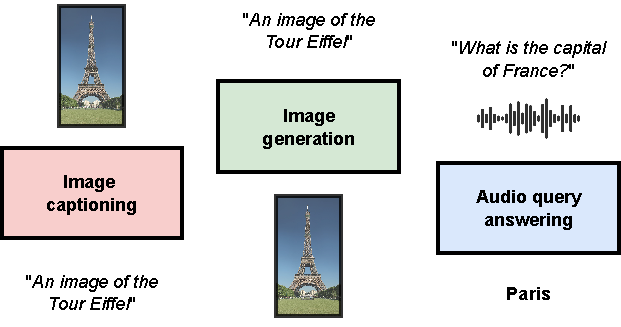
\includegraphics[width=0.6\textwidth]{images/examples.pdf}
    \caption{Большинство задач можно классифицировать на основе желаемого входа-выхода: {\color{drawgreen}генерация изображений} требует изображения (\textit{упорядоченной сетки} пикселей) из текста (\textit{последовательности} символов), в то время как обратная задача ({\color{drawred}создание подписей к изображениям}) — это проблема генерации подписи из изображения. В качестве другого примера, {\color{drawblue}ответы на аудиозапросы} требуют текста из аудио (другой \textit{упорядоченной} последовательности, на этот раз числовой). Удивительно, но дизайн моделей следует схожим спецификациям во всех случаях.}
    \label{fig:examples}
\end{figure}

В общем, обучение — это задача \textbf{поиска}. Мы начинаем с определения программы с большим количеством \textit{степеней свободы} (которые мы называем параметрами) и манипулируем параметрами до тех пор, пока производительность модели не станет удовлетворительной. Чтобы сделать эту идею практичной, нам нужны эффективные способы поиска оптимальной конфигурации даже при наличии миллионов (или миллиардов, или триллионов) таких параметров. Как следует из названия, \textbf{дифференцируемые модели} делают это, ограничивая выбор модели дифференцируемыми компонентами, т.е. математическими функциями, которые мы можем дифференцировать. Возможность вычислить производную многомерной функции (градиент) означает знание того, что произойдет, если мы немного изменим их параметры, что, в свою очередь, приводит к автоматическим процедурам их оптимизации (в первую очередь, \textbf{автоматическому дифференцированию} и \textbf{градиентному спуску}). Описание этой схемы является темой первой части книги (Часть \ref{part:compass_and_needle}, \textbf{Компас и игла}), с Главы \ref{chap:preliminaries} по Главу \ref{chap:automatic_differentiation}.

Рассматривая нейронные сети как просто композиции дифференцируемых примитивов, мы можем задать два основных вопроса (Рисунок \ref{fig:differentiable_programming}): во-первых, какие \textbf{типы данных} мы можем обрабатывать в качестве входов или выходов? И во-вторых, какие примитивы мы можем использовать? Дифференцируемость — это сильное требование, которое не позволяет нам напрямую работать со многими стандартными типами данных, такими как символы или целые числа, которые являются принципиально \textit{дискретными} и, следовательно, разрывными. Напротив, мы увидим, что дифференцируемые модели могут легко работать с более сложными данными, представленными в виде больших массивов (которые мы будем называть \textbf{тензорами}) чисел, таких как изображения, которыми можно алгебраически манипулировать с помощью базовых композиций линейных и нелинейных преобразований.

Во второй части книги мы сосредоточимся на прототипическом примере дифференцируемого компонента — \textbf{свёрточном} операторе (Часть \ref{part:a_strange_land}, с Главы \ref{chap:cnns} до Главы \ref{chap:deep_cnns}). Свёртки можно применять всякий раз, когда наши данные могут быть представлены упорядоченной последовательностью элементов: к ним относятся, среди прочего, аудио, изображения, текст и видео. Попутно мы также представим ряд полезных техник для проектирования \textit{глубоких} (т.е. состоящих из многих последовательных шагов) моделей, а также несколько важных идей, таких как \textbf{токенизация текста}, \textbf{авторегрессионная} генерация последовательностей и \textbf{причинное} моделирование, которые составляют основу современных БЯМ.

\begin{SCfigure}
    \centering
    \hspace{1em}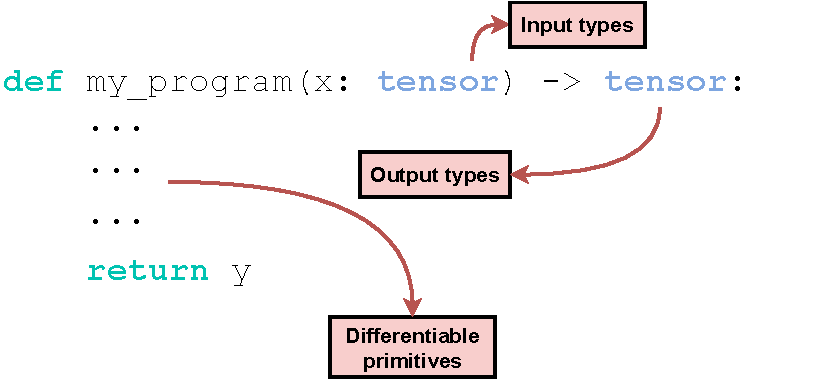
\includegraphics[width=0.6\textwidth]{images/differentiable_programming.pdf}
    \caption{Нейронные сети — это последовательности дифференцируемых \textbf{примитивов}, которые оперируют структурированными массивами (\textbf{тензорами}): каждый примитив можно классифицировать на основе его сигнатуры ввода/вывода, которая, в свою очередь, определяет правила их композиции.}
    \label{fig:differentiable_programming}
\end{SCfigure}

Третья часть книги (Часть \ref{part:down_the_rabbit_hole}, \textbf{Вниз по кроличьей норе}) продолжает наше исследование дифференцируемых моделей, рассматривая альтернативные дизайны для множеств (в первую очередь, слои \textbf{внимания} и модели \textbf{трансформеров} в Главах \ref{chap:transformers} и \ref{chap:transformers_in_practice}), графов (Глава \ref{chap:gnns}) и, наконец, рекуррентных слоев для временных последовательностей (Глава \ref{chap:rnns}).

Книга дополнена веб-сайтом\footnote{\url{https://sscardapane.it/alice-book}}, где я собираю дополнительные главы и материалы по интересующим темам, которые не сосредоточены на конкретном типе данных, включая \textbf{генеративное моделирование}, \textbf{условные вычисления}, \textbf{трансферное обучение} и \textbf{объяснимость}. Эти главы носят более исследовательский характер и могут быть прочитаны в любом порядке. Надеюсь, они станут частью второго тома, если позволит время.
%
\section*{Что такое «дифференцируемое программирование»?}

Нейронные сети имеют долгую и богатую историю. Само название является отсылкой к ранним попыткам моделирования (биологических) нейронов в 20-м веке, и подобная терминология осталась широко распространенной: чтобы соответствовать существующим фреймворкам, в последующих главах мы можем ссылаться на \textit{нейроны}, \textit{слои} или, например, \textit{активации}. После нескольких волн интереса, период с 2012 по 2017 год ознаменовался беспрецедентным ростом сложности сетей, стимулированным крупномасштабными бенчмарками и соревнованиями, в первую очередь \textbf{ImageNet Large Scale Visual Recognition Challenge} (ILSVRC), который мы рассмотрим в Главе \ref{chap:deep_cnns}. Вторая крупная волна интереса пришла с введением \textbf{трансформеров} (Глава \ref{chap:transformers}) в 2017 году: так же, как компьютерное зрение было захвачено свёрточными моделями несколькими годами ранее, обработка естественного языка была захвачена трансформерами за очень короткий период. Дальнейшие усовершенствования в эти годы были сделаны для видео, графов (Глава \ref{chap:gnns}) и аудио, кульминацией чего стал нынешний ажиотаж вокруг БЯМ, мультимодальных сетей и генеративных моделей.\footnote{Это не место для полного исторического обзора современных нейронных сетей; заинтересованному читателю я рекомендую \cite{metz2022genius} в качестве отличной отправной точки.}

Этот период сопровождался быстрой эволюцией терминологии, от \textbf{коннекционизма} 80-х годов \cite{rumelhart1986general} до использования \textbf{глубокого обучения} для обозначения современных сетей в противовес меньшим, \textit{более мелким} моделям прошлого \cite{bengio2009learning,lecun2015deep}. Несмотря на это, все эти термины остаются неумолимо расплывчатыми, потому что современные (искусственные) сети почти не имеют сходства с биологическими нейронными сетями и неврологией \cite{zador2023catalyzing}. Глядя на современные нейронные сети, их существенной характеристикой является то, что они состоят из дифференцируемых блоков: по этой причине в этой книге я предпочитаю термин \textbf{дифференцируемые модели}, когда это возможно. Рассмотрение нейронных сетей как дифференцируемых моделей напрямую ведет к более широкой теме \textbf{дифференцируемого программирования}, новой дисциплины, которая сочетает в себе информатику и оптимизацию для более широкого изучения дифференцируемых компьютерных программ \cite{blondel2024elements}.\footnote{Как и многих, меня вдохновил «манифест», опубликованный Я. Лекуном на Facebook в 2018 году: \url{https://www.facebook.com/yann.lecun/posts/10155003011462143}. За связь между нейронными сетями и программированием с открытым исходным кодом (и разработкой) я также благодарен второму манифесту, опубликованному К. Раффелем в 2021 году: {\url{https://colinraffel.com/blog/a-call-to-build-models-like-we-build-open-source-software.html}}.}

Путешествуя по этой стране дифференцируемых моделей, мы также путешествуем по истории: основные концепции численной оптимизации линейных моделей методом градиентного спуска (рассмотренные в Главе \ref{chap:linear_models}) были известны по крайней мере с XIX века \cite{stigler1981gauss}; так называемые «полносвязные сети» в том виде, в котором мы их используем позже, можно отнести к 1980-м годам \cite{rumelhart1986general}; свёрточные модели были известны и использовались уже в конце 90-х \cite{lecun1998gradient}.\footnote{Историю НС до этого периода через интервью с некоторыми из главных действующих лиц см. в \cite{anderson2000talking}; для большой субъективной истории есть также \textit{аннотированная история нейронных сетей} Ю. Шмидхубера: \url{https://people.idsia.ch/~juergen/deep-learning-history.html}.}

\begin{figure}
    \centering
    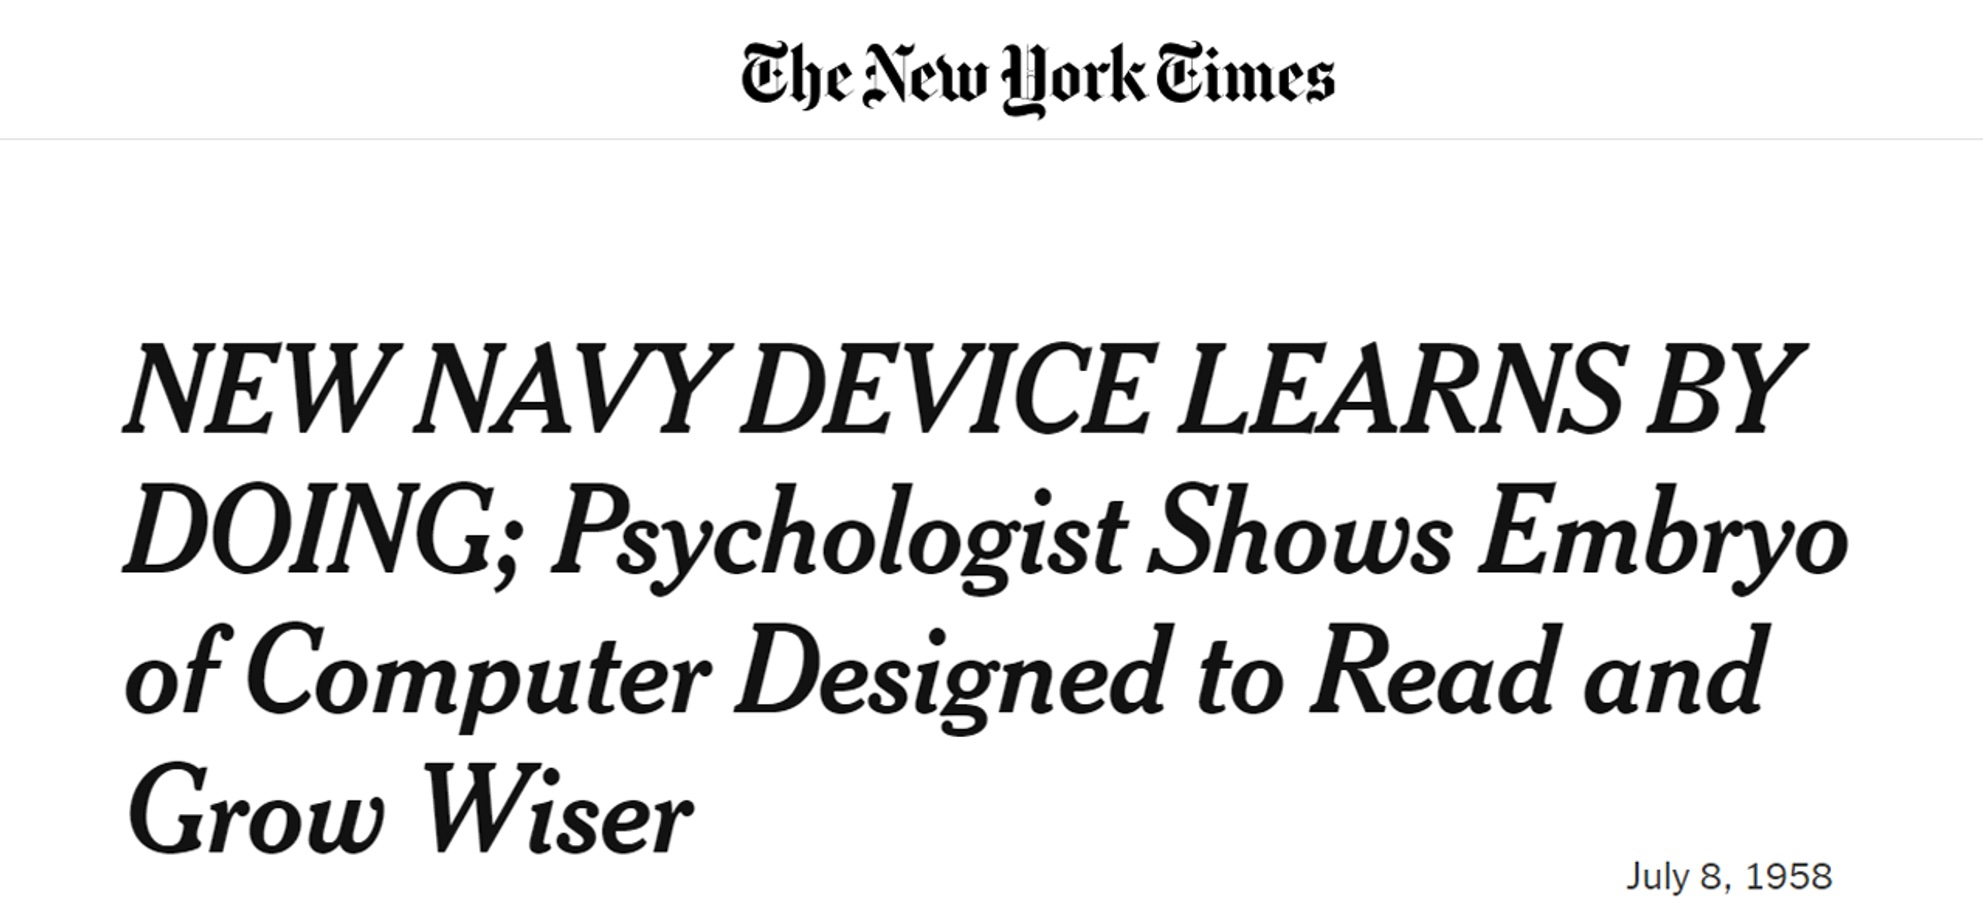
\includegraphics[width=0.7\textwidth]{images/Rosenblatt_cut.jpg}
    \caption*{Ажиотаж вокруг ИИ - только это 1958 год, и американский психолог Фрэнк Розенблатт привлек значительное внимание СМИ своими исследованиями «перцептронов», одного из первых рабочих прототипов нейронных сетей.}
\end{figure}

Хотя у нас нет места для углубленного рассмотрения всех возможных тем (также из-за того, как быстро развивается исследование), я надеюсь, что книга предоставит достаточно материала, чтобы позволить читателю легко ориентироваться в самой последней литературе.

\section*{Обозначения и символы}
\label{sec:notation}

\begin{figure}
    \centering
    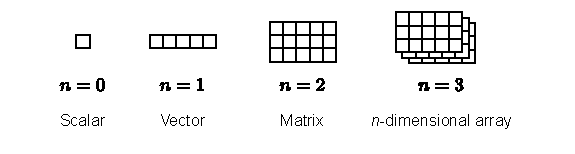
\includegraphics[width=0.9\textwidth]{images/Tensors.pdf}
    \caption*{Основные типы данных: скаляры, векторы, матрицы и общие $n$-мерные массивы. Мы используем название \textbf{тензоры} для их обозначения. $n$ называется \textbf{рангом} тензора. Мы показываем вектор как строку для удобочитаемости, но в тексте мы предполагаем, что все векторы являются \textit{векторами-столбцами}.}
\end{figure}

Основным типом данных при работе с дифференцируемыми моделями является \textbf{тензор},\footnote{В научной литературе тензоры имеют более точное определение как мультилинейные операторы \cite{lim2021tensors}, в то время как объекты, которые мы используем в книге, являются более простыми многомерными массивами. Хотя технически это неправильное название, использование \textit{тензора} настолько широко распространено, что мы придерживаемся этой конвенции здесь.} который мы определяем как $n$-мерный массив объектов, обычно вещественных чисел. С необходимыми извинениями перед любым математиком, читающим нас,\footnote{Предполагая, что кто-то нас действительно читает.} мы называем $n$ \textbf{рангом} тензора. Обозначения в книге варьируются в зависимости от $n$:
%
\begin{itemize}
    \item А single-item tensor ($n=0$) — это просто одно значение (\textbf{скаляр}). Для скаляров мы используем строчные буквы, такие как $x$ или $y$. \footnote{Если вам интересно, скаляры названы так потому, что их можно записать как скалярные кратные единицы. Также я обещаю сократить количество сносок с этого момента.}
    \item Столбцы значений ($n=1$) называются \textbf{векторами}. Для векторов мы используем строчный жирный шрифт, например $\mathbf{x}$. Соответствующий вектор-строка обозначается как $\mathbf{x}^\top$, когда нам нужно их различать. Мы также можем игнорировать транспонирование для удобочитаемости, если форма ясна из контекста.
    \item Прямоугольные массивы значений ($n=2$) называются \textbf{матрицей}. Мы используем прописной жирный шрифт, например $\mathbf{X}$ или $\mathbf{Y}$.
    \item Для $n > 2$ специального обозначения не используется. Мы избегаем каллиграфических символов, таких как $\mathcal{X}$, которые мы оставляем для множеств или распределений вероятностей.
\end{itemize}
%
Для работы с тензорами мы используем различные стратегии индексации, описанные подробнее в Разделе \ref{sec:linear_algebra}. В большинстве случаев понимание алгоритма или операции сводится к пониманию формы каждого задействованного тензора. Чтобы кратко обозначить форму, мы используем следующую нотацию:
%
$$
X \sim(b,h,w,3)
$$
%
Это тензор ранга $4$ с формой $(b,h,w,3)$. Некоторые измерения могут быть предварительно заданы (например, $3$), в то время как другие измерения могут быть обозначены переменными. Мы используем тот же символ для обозначения выборки из распределения вероятностей, например, $\varepsilon \sim \mathcal{N}(0,1)$, но мы делаем это редко, и значение символа всегда должно быть ясно из контекста. Следовательно, $\mathbf{x} \sim (d)$ заменит более распространенное $\mathbf{x} \in \mathbb{R}^d$, и аналогично для $\mathbf{X} \sim (n,d)$ вместо $\mathbf{X} \in \mathbb{R}^{n \times d}$.
%
Наконец, мы можем захотеть ограничить элементы тензора, для чего мы используем специальное обозначение:
%
\begin{enumerate}
    \item $\mathbf{x} \sim \text{Binary}(c)$ обозначает тензор только с двоичными значениями, т.е. элементами из множества $\left\{0,1\right\}$.
    \item $\mathbf{x} \sim \Delta(a)$ обозначает вектор, принадлежащий так называемому \textbf{симплексу}, т.е. $x_i \ge 0$ и $\sum_i x_i = 1$. Для тензоров более высокого ранга, например, $\mathbf{X} \sim \Delta(n,c)$, мы предполагаем, что нормализация применяется по последнему измерению (например, в этом случае каждая строка $\mathbf{X}_i$ принадлежит симплексу).
\end{enumerate}
%
Дополнительные обозначения вводятся в каждой главе по мере необходимости. У нас также есть несколько символов сбоку: 

\begin{itemize}
\item  \addbottle \textbf{Бутылка} для выделения некоторых определений. У нас много определений, особенно в ранних главах, и мы используем этот символ, чтобы визуально выделить самые важные.
\item \addclock \textbf{Часы} для разделов, которые, по нашему мнению, имеют решающее значение для понимания остальной части книги — пожалуйста, не пропускайте их!
\item \addteacup Напротив, \textbf{чашка чая} для более расслабленных разделов — они, как правило, носят дискурсивный характер и в основном необязательны по отношению к остальной части книги.
\end{itemize}

\section*{Последние мысли перед отправлением}

Книга возникла из моего желания придать стройную форму лекциям, которые я подготовил для курса под названием \textbf{Нейронные сети для приложений в науке о данных}, который я преподаю на магистерской программе по науке о данных в Римском университете Сапиенца в течение нескольких лет. Основные главы книги составляют основную часть курса, в то время как остальные главы — это темы, которые я рассматриваю время от времени в зависимости от года. Некоторые части были дополнены дополнительными курсами, которые я преподавал (или собираюсь преподавать), включая части \textbf{Нейронных сетей} для компьютерной инженерии, введение в машинное обучение для телекоммуникационной инженерии, а также несколько учебных пособий, курсов для аспирантов и летних школ на протяжении многих лет.

Уже существует ряд отличных (и недавних) книг по теме современных, глубоких нейронных сетей, включая \cite{prince2023understanding, zhang2023dive,bishop2024deep,fleuret2023little,hardt2022patterns}. Эта книга охватывает схожее содержание со всеми из них в начале, в то время как изложение и некоторые дополнительные части (или несколько разделов в продвинутых главах) пересекаются меньше, и они в основном зависят от моих исследовательских интересов. Я надеюсь, что смогу предоставить дополнительную (и дополняющую) точку зрения на существующий материал.

% As a rule, I believe it is important to understand why and how certain equations come to be, especially in a field such as neural networks, where untold questions must be answered with \textit{because it works best this way} or \textit{historically it has been like this}. Hence, I have tried to provide a simple formalism with enough rigor, while giving insights when possible into each and every concept that I introduce. In general, I have avoided theorems, proofs, or analyses of convergence or approximation. There are much better resources in this regard than I can provide.

Как следует из моего выбора названия, понимание дифференцируемых \textit{программ} происходит как из теории, так и из кодирования: существует постоянное взаимодействие между тем, как мы проектируем модели и как мы их реализуем, причем такие темы, как автоматическое дифференцирование, являются лучшим примером. Нынешнее возрождение нейронных сетей (примерно с 2012 года) во многом можно отнести к доступности мощных программных библиотек, начиная от Theano \cite{al2016theano} до Caffe, Chainer, а затем непосредственно к современным итерациям TensorFlow, PyTorch и JAX, среди прочих. Я стараюсь по возможности связывать обсуждение с концепциями из существующих программных фреймворков, с акцентом на PyTorch и JAX. Однако эта книга не является руководством по программированию, и я отсылаю к документации библиотек для полного введения в каждую из них.

Прежде чем двигаться дальше, я хотел бы перечислить еще несколько вещей, которыми эта книга \textit{не является}. Во-первых, я попытался выбрать несколько концепций, которые являются одновременно (а) распространенными сегодня и (б) достаточно общими, чтобы быть полезными в ближайшем будущем. Однако я не могу предвидеть будущее и не стремлюсь к полноте, и несколько частей этих глав могут быть неполными или устаревшими к тому времени, как вы их прочтете. Во-вторых, для каждой концепции я стараюсь привести несколько примеров вариаций, существующих в литературе (например, от пакетной нормализации до послойной нормализации). Однако имейте в виду, что существуют сотни других: для этого я приглашаю вас к исследованию множества страниц \href{http://paperswithcode.com}{Papers With Code}. Наконец, это книга об основных компонентах дифференцируемых моделей, но их реализация в масштабе (и обеспечение их работы) требует как инженерной изощренности, так и (немного) интуиции. Я мало касаюсь аппаратной стороны, а для последней ничто не заменит опыт и субъективные посты в блогах.\footnote{См., например, этот пост в блоге А. Карпати: \url{http://karpathy.github.io/2019/04/25/recipe/}, или его недавнюю серию видео \textbf{Zero to Hero}: \url{https://karpathy.ai/zero-to-hero.html}.}

\section*{Благодарности}
%
Equations' coloring is thanks to the beautiful {\footnotesize\verb+st--/annotate-equations+}
package.\footnote{\url{https://github.com/st--/annotate-equations/tree/main}} Color images of Alice in Wonderland and the black and white symbols in the margin are all licensed from Shutterstock.com. The images of Alice in Wonderland in the figures from the main text are reproductions from the original Arthur Rackham's 1907 illustrations, thanks to Wikimedia.\footnote{\url{ https://commons.wikimedia.org/wiki/Category:Alice\%27s\_adventures\_in\_Wonderland\_(Rackham,\_1907)}} I thank Roberto Alma for extensive feedback on a previous draft of the book and for encouraging me to publish the book. I also thank Corrado Zoccolo and Emanuele Rodolà for providing corrections and suggestions to the current version, and everyone who provided me feedback via email.